\section{Próbki zaburzone}
Teraz chciałbym jeszcze trochę poeksperymentować z treścią reguł poddawanych analizie i przyjrzeć im się pod kątem odporności na różnego typu zaburzenia takie jak np. literówki czy niepoprawna struktura reguł. 
\subsection{Literówki i nieznane słowa}
Jako oznaczenie akcji, które mają zostać wykonane wprowadzam określenia, które nigdy nie pojawiły się w danych uczących. 
\\ \\
\fbox{\begin{minipage}{40em}
		\textit{Jeżeli data\_rejestracji\_badania jest większa niż '01-01-2019' i data\_rejestracji\_badania jest mniejsza od '01-04-2019' wtedy \textbf{zaprezentuj komunikat} "Badanie podlega refundacji", w przeciwnym wypadku \textbf{wyrzuć błąd} "Badanie nie może zostać zarejestrowane" . }
\end{minipage}}
\\ \\

\begin{figure}[H]
	\centering
	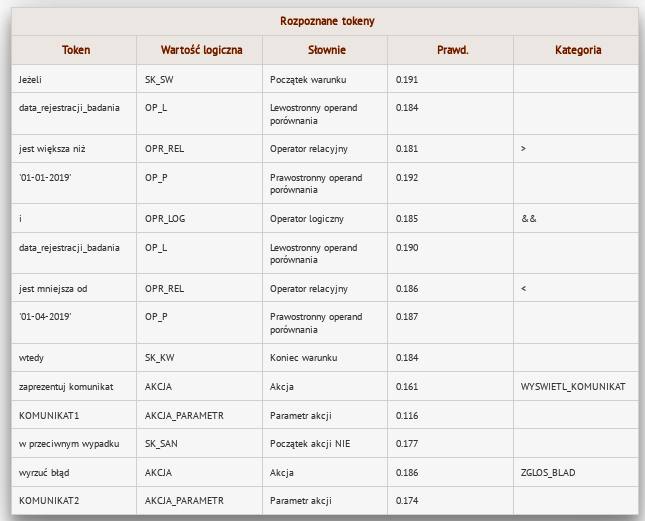
\includegraphics[scale=0.8]{img/app-eksperymenty/p5-1.png}
\end{figure}

Jak widać algorytm znowu sobie poradził,  niestety nie jest to jednak regułą. Tolerancja na błędy pojawia się tylko w niewielkim zakresie. Może jest to związane z niskimi prawdopodobieństwami, z jakimi algorytm rozpoznaje moje encje. 

Dla przykładu wprowadźmy jeszcze jedną modyfikację, tym razem wyrażenie ,,jest mniejsza od'' zamienię na  ,,jest mniejsz od''.
\\ \\
\fbox{\begin{minipage}{40em}
		\textit{Jeżeli data\_rejestracji\_badania jest większa niż '01-01-2019' i data\_rejestracji\_badania \textbf{jest mniejs od} '01-04-2019' wtedy \textbf{zaprezentuj komunikat} "Badanie podlega refundacji", w przeciwnym wypadku \textbf{wyrzuć błąd} "Badanie nie może zostać zarejestrowane" . }
\end{minipage}}
\\ \\

I ta niewielka zmiana wystarczy by algorytm zadziałał źle. Bo chociaż z jednej strony uznał, że fraza ta jest operatorem relacyjnym, to dokonał złej jego kategoryzacji, bo zamiast przypisać go do kategorii ,,<'', trafił on do kategorii ,,>'', niestety z punktu widzenia jakości wygenerowanego kodu, pomyłka ma zasadnicze znaczenie.
\begin{figure}[H]
	\centering
	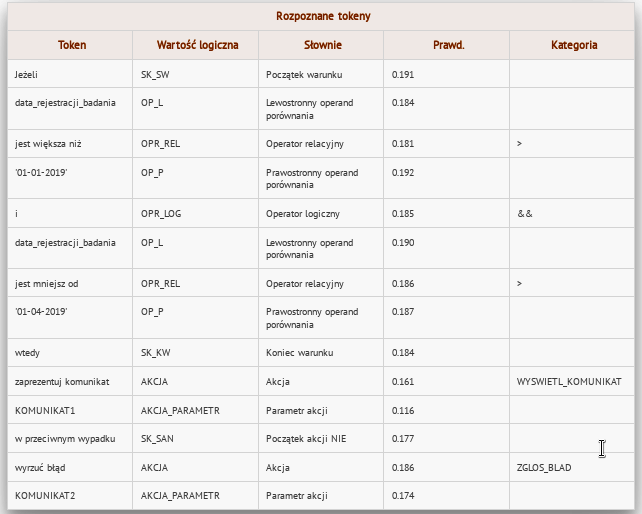
\includegraphics[scale=0.8]{img/app-eksperymenty/p5-2.png}
\end{figure}

\subsection{Zaburzenia struktury i niezgodność z abstrakcyjnym modelem reguły}
Spróbujmy teraz przyjrzeć się reakcji algorytmu na dużo bardziej złożone zaburzenie - niezgodność z przyjetym schematerm reguły. Załóżmy, że z reguły znika słowo ,,WTEDY''.
\\ \\
\fbox{\begin{minipage}{40em}
		\textit{Jeżeli data\_rejestracji\_badania jest większa niż '01-01-2019' i data\_rejestracji\_badania jest mniejsza od '01-04-2019' wyświetl komunikat "Badanie podlega refundacji", w przeciwnym wypadku zgłoś błąd "Badanie nie może zostać zarejestrowane" .}
\end{minipage}}
\\ \\

\begin{figure}[H]
	\centering
	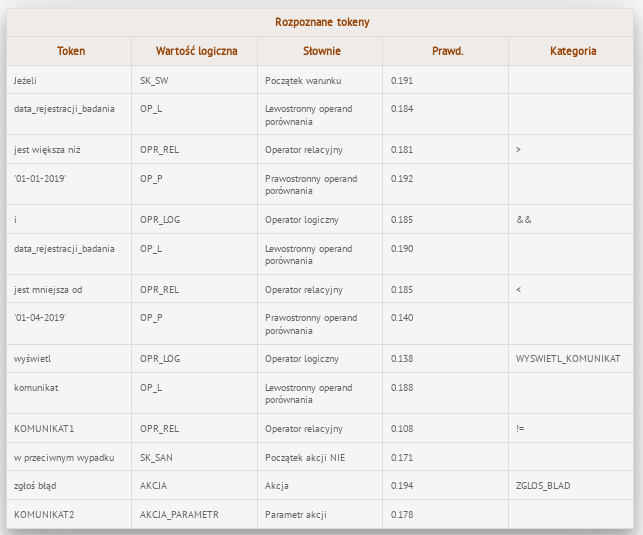
\includegraphics[scale=0.8]{img/app-eksperymenty/p6-1.png}
\end{figure}
Jak można łatwo zauważyć, w tym przypadku algorytm sobie nie poradził. W poszukiwaniu znanego mu wzorca dokonał złych przyporządkowań. Ciekawe natomiast jest to, że mimo pomyłki sekcji rozpoznawania akcji TAK, części reguły leżące poza nią , w sekcji akcji NIE zostały rozpoznane prawidłowo.
\subsection{Podsumowanie}
Niestety w zakresie uodpornienia algorytmu na pomyłki i niezgodności z założoną strukturą pozostało wiele do zrobienia. Stosunkowo niewielkie pomyłki prowadzą do złej interpretacji reguły i wygenerowania wadliwego kodu.